\begin{figure}[H]
\centering
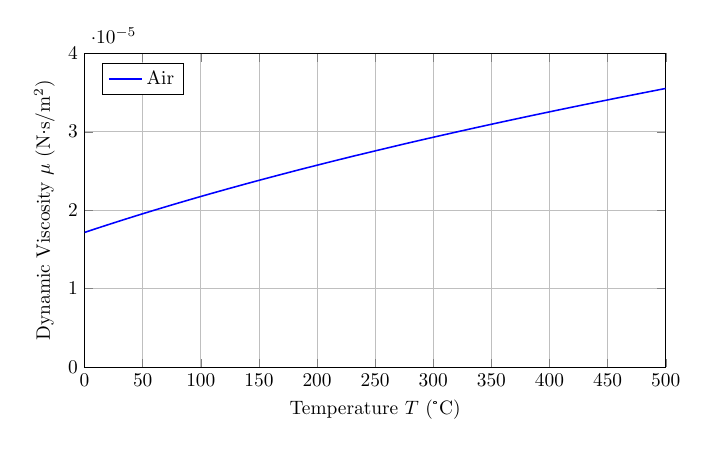
\begin{tikzpicture}[scale=0.7]
    \begin{axis}[
        width=\textwidth,
        height=0.6\textwidth,
        xlabel={Temperature $T$ (°C)},
        ylabel={Dynamic Viscosity $\mu$ (N·s/m$^2$)},
        xmin=0, xmax=500,
        ymin=0, ymax=4e-5,
        domain=0:500,
        grid=both,
        legend pos=north west,
    ]
        % Sutherland's formula parameters for Air
        \addplot [
            thick,
            blue,
            samples=200
        ]
        {(1.716e-5) * ((273+x)/273)^(3/2) * (273+111)/(273+x+111)};
        \addlegendentry{Air}
    \end{axis}
\end{tikzpicture}
\end{figure}
